\subsection{FFT Noise}
There are two kinds of noise in the data we obtained, random noise and coherent noise.
Random noise is the noise which exists in each anode channel.
Coherent noise is in each board.
The pseudo noise we implemented in Monte Carlo simulation is composed of random and coherent noise by this reason.

Random noise is generated from FFT(Fast Fourier Transform) distribution of real data. Figure \ref{example10ch} shows an example of FFT distribution.

Coherent noise is generated board by board as the noise scale in the real data we obtained.
The noise scale is defined as a root mean square of pedestal, minimum noise scale is about 3 and maximum noise scale is about 10 in the data.

The ratio of random and coherent noise is 1:1 as equation \ref{PseudoNoise}.
Figure \ref{DATAnoise} shows real data noise and Fig.\ref{MCnoise} shows pseudo noise we implemented in Monte Carlo simulation.
\begin{equation}
  Pseudo\,Noise = \frac{Random\,Noise + Coherent\,Noise}{2}
  \label{PseudoNoise}
\end{equation}

\begin{figure}[!htb]
  \centering
  \centering
  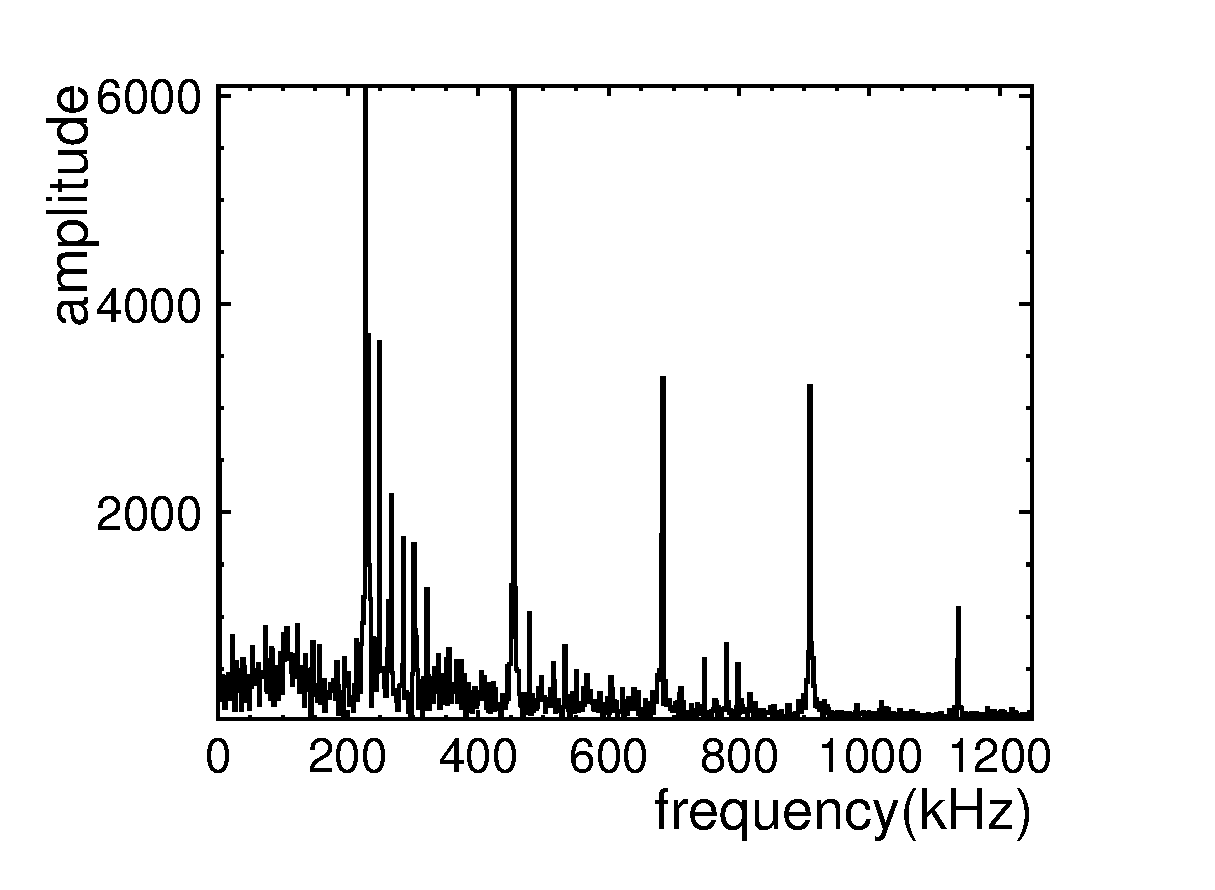
\includegraphics[width=10cm,clip]{./fig/FFTdist.eps}
  \caption{An example distribution of frequency}
  \label{example10ch}
\end{figure}
%\begin{figure}[!htb]
%  \centering
%  \centering
%  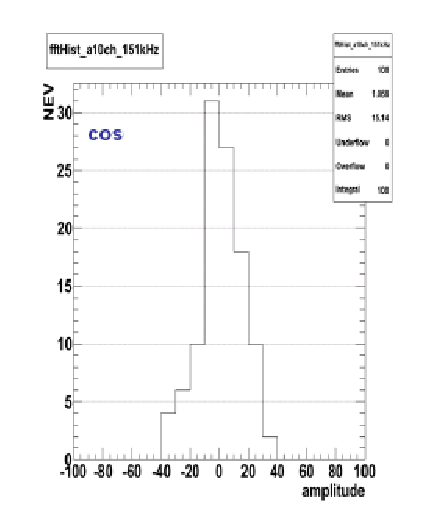
\includegraphics[width=11cm,clip]{./fig/cos.eps}
%  \caption{An example of distribution of amplitude}
%  \label{ampDist}
%\end{figure}
%\begin{figure}[!htb]
%  \centering
%  \centering
%  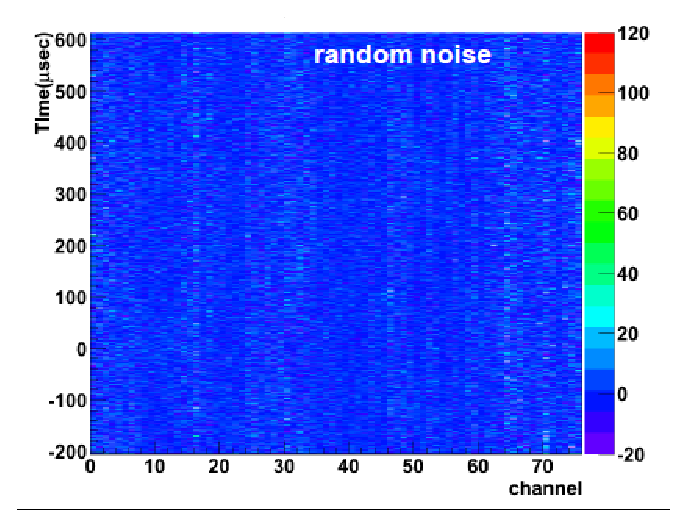
\includegraphics[width=11cm,clip]{./fig/randomnoise.eps}
%  \caption{Random noise}
%  \label{randomNoise}
%\end{figure}
\begin{figure}[!htb]
\begin{minipage}{0.5\hsize}
  \centering
  \includegraphics[width=7cm,clip]{./fig/DATAnoise.eps}
  \caption{Data noise}
  \label{DATAnoise}
\end{minipage}
\begin{minipage}{0.5\hsize}
  \centering
  \includegraphics[width=7cm,clip]{./fig/MCnoise.eps}
  \caption{Pseudo noise(Noise simulation)}
  \label{MCnoise}
\end{minipage}
\end{figure}
%\begin{figure}[!htb]
%  \centering
%  \centering
%  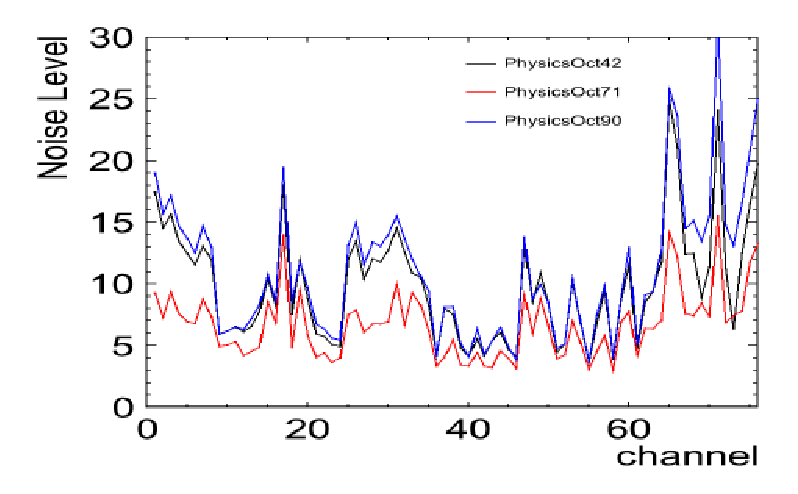
\includegraphics[width=11cm,clip]{./fig/scaling.eps}
%  \caption{Noise level}
%  \label{scaling}
%\end{figure}